\documentclass{article}
\usepackage[margin=1in]{geometry}
\usepackage{amsmath,amsthm,amssymb}
\usepackage{bbm,enumerate,mathtools}
\usepackage{tikz,pgfplots}
\usepackage{chessboard}
\usepackage[hidelinks]{hyperref}
\usepackage{multicol} % Problem 35

\newenvironment{question}{\begin{trivlist}\item[\textbf{Question.}]}{\end{trivlist}}
\newenvironment{note}{\begin{trivlist}\item[\textbf{Note.}]}{\end{trivlist}}
\newenvironment{references}{\begin{trivlist}\item[\textbf{References.}]}{\end{trivlist}}
\newenvironment{related}{\begin{trivlist}\item[\textbf{Related.}]\end{trivlist}\begin{enumerate}}{\end{enumerate}}


\begin{document}
\rating{3}{2}
Consider all of the shapes that can be made with a rubber band and a rubber
hand.

\begin{figure}[!h]
  \centering
  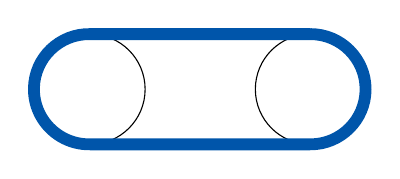
\begin{tikzpicture}[scale=0.7]
    \draw (0,0) circle (1);
    \draw (4,0) circle (1);
    \draw[line width=0.15cm, draw={rgb:green,1;blue,2}] 
      (0,1) arc (89:271:1)
      (0,1)--(4,1)
      (4,-1) arc (270:450:1)
      (0,-1)--(4,-1)
    ;
  \end{tikzpicture}
  \hspace{0.5cm}
  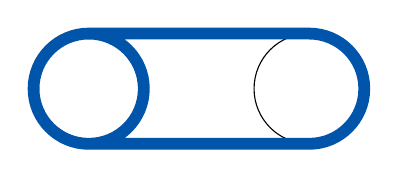
\begin{tikzpicture}[scale=0.7]
    \draw (0,0) circle (1);
    \draw (4,0) circle (1);
    \draw[line width=0.15cm, draw={rgb:green,1;blue,2}] 
      (0,1) arc (90:450:1)
      (0,1)--(4,1)
      (0,-1)--(4,-1)
      (4,-1) arc (270:450:1)
    ;
  \end{tikzpicture}
  \hspace{0.5cm}
  
\begin{tikzpicture}[scale=0.7]
    \draw (0,0) circle (1);
    \draw (4,0) circle (1);
    \draw[line width=0.15cm, draw={rgb:green,1;blue,2}] 
      (0,1) arc (90:450:1)
      (0,1)--(4,1)
      (0,-1)--(4,-1)
      (5,0) arc (0:361:1)
    ;
  \end{tikzpicture}
  \\~\\
  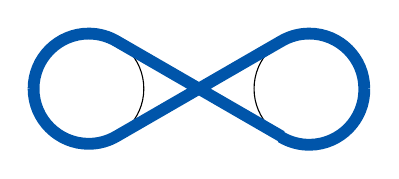
\begin{tikzpicture}[scale=0.7]
    \draw (0,0) circle (1);
    \draw (4,0) circle (1);
    \draw[line width=0.15cm, draw={rgb:green,1;blue,2}] 
      (-1,0) arc (180:59:1)
      (-1,0) arc (180:301:1)
      (5,0) arc (0:121:1)
      (5,0) arc (1:-121:1)
      (0.5,{-1.5/sqrt(3)})--(3.5, {1.5/sqrt(3)})
      (0.5,{1.5/sqrt(3)})--(3.5, {-1.5/sqrt(3)})
    ;
  \end{tikzpicture}
  \hspace{0.5cm}
  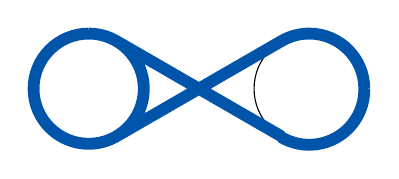
\begin{tikzpicture}[scale=0.7]
    \draw (0,0) circle (1);
    \draw (4,0) circle (1);
    \draw[line width=0.15cm, draw={rgb:green,1;blue,2}] 
      (0,1) arc (90:450:1)
      (5,0) arc (0:121:1)
      (5,0) arc (1:-121:1)
      (0.5,{-1.5/sqrt(3)})--(3.5, {1.5/sqrt(3)})
      (0.5,{1.5/sqrt(3)})--(3.5, {-1.5/sqrt(3)})
    ;
  \end{tikzpicture}
  \hspace{0.5cm}
  
\begin{tikzpicture}[scale=0.7]
    \draw (0,0) circle (1);
    \draw (4,0) circle (1);
    \draw[line width=0.15cm, draw={rgb:green,1;blue,2}] 
      (0,1) arc (90:450:1)
      (5,0) arc (0:361:1)
      (0.5,{-1.5/sqrt(3)})--(3.5, {1.5/sqrt(3)})
      (0.5,{1.5/sqrt(3)})--(3.5, {-1.5/sqrt(3)})
    ;
  \end{tikzpicture}
  \\~\\
  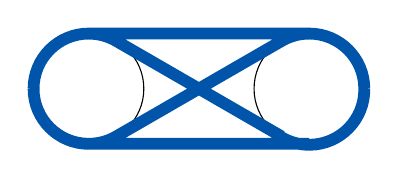
\begin{tikzpicture}[scale=0.7]
    \draw (0,0) circle (1);
    \draw (4,0) circle (1);
    \draw[line width=0.15cm, draw={rgb:green,1;blue,2}] 
      (-1,0) arc (180:59:1)
      (-1,0) arc (180:301:1)
      (0,1)--(4,1)
      (0,-1)--(4,-1)
      (5,0) arc (0:121:1)
      (5,0) arc (1:-121:1)
      (0.5,{-1.5/sqrt(3)})--(3.5, {1.5/sqrt(3)})
      (0.5,{1.5/sqrt(3)})--(3.5, {-1.5/sqrt(3)})
    ;
  \end{tikzpicture}
  \hspace{0.5cm}
  
\begin{tikzpicture}[scale=0.7]
    \draw (0,0) circle (1);
    \draw (4,0) circle (1);
    \draw[line width=0.15cm, draw={rgb:green,1;blue,2}] 
      (0,1) arc (90:450:1)
      (0,1)--(4,1)
      (0,-1)--(4,-1)
      (5,0) arc (0:121:1)
      (5,0) arc (1:-121:1)
      (0.5,{-1.5/sqrt(3)})--(3.5, {1.5/sqrt(3)})
      (0.5,{1.5/sqrt(3)})--(3.5, {-1.5/sqrt(3)})
    ;
  \end{tikzpicture}
  \hspace{0.5cm}
  
\begin{tikzpicture}[scale=0.7]
    \draw (0,0) circle (1);
    \draw (4,0) circle (1);
    \draw[line width=0.15cm, draw={rgb:green,1;blue,2}] 
      (0,1) arc (90:450:1)
      (0,1)--(4,1)
      (5,0) arc (0:361:1)
      (0,-1)--(4,-1)
      (0.5,{-1.5/sqrt(3)})--(3.5, {1.5/sqrt(3)})
      (0.5,{1.5/sqrt(3)})--(3.5, {-1.5/sqrt(3)})
    ;
  \end{tikzpicture}
  \caption{
    There are (at least) 9 ways to weave a rubber band between two fingers up to
    reflection/rotation.
  }
\end{figure}

\begin{question}
  How many figures can be made with $n$ fingers and a rubber band?
\end{question}
\begin{related}
  \item Is there an analog in higher dimensions?
  \item What if all fingers must be aligned?
  \item What if all fingers must be on the corners of an $n$-gon?
\end{related}
\end{document}
